\documentclass[12pt, preprint]{aastex}

\usepackage{subfigure}
\usepackage{color}
\usepackage{hyperref}
\usepackage{url}
\usepackage{natbib}

\newcommand{\project}[1]{\textsl{#1}}
\newcommand{\cpm}{\project{CPM}}
\newcommand{\cpmdiff}{\project{CPM Difference Imaging}}
\newcommand{\class}{\project{the classical difference imaging}}
\newcommand{\kepler}{\project{Kepler}}
\newcommand{\KTCZ}{\project{K2 Campaign 0}}
\newcommand{\todo}[1]{\textbf{#1}}
\newcommand{\set}[1]{\mathcal{#1}}

\graphicspath{{figures/}}

\bibliographystyle{apj}
\definecolor{linkcolor}{rgb}{0,0,0.5}
\hypersetup{colorlinks=true,linkcolor=linkcolor,citecolor=linkcolor,
            filecolor=linkcolor,urlcolor=linkcolor}

\begin{document}

\title{Pixel-level model for image differencing in variability campaigns}
\author{%
  Dun~Wang\altaffilmark{\ref{CCPP}},
  David~W.~Hogg\altaffilmark{\ref{CCPP},\ref{CDS},\ref{MPIA},\ref{email}},
  Daniel~Foreman-Mackey\altaffilmark{\ref{UW},\ref{SF}}
  }
\newcounter{address}
\setcounter{address}{1}
\altaffiltext{\theaddress}{\stepcounter{address}\label{CCPP}%
  Center for Cosmology and Particle Physics, Department of Physics, New York University}
\altaffiltext{\theaddress}{\stepcounter{address}\label{CDS}%
  Center for Data Science, New York University}
\altaffiltext{\theaddress}{\stepcounter{address}\label{MPIA}%
  Max-Planck-Institut f\"ur Astronomie, Heidelberg, Germany}
\altaffiltext{\theaddress}{\stepcounter{address}\label{email}%
  To whom correspondence should be addressed; \texttt{<david.hogg@nyu.edu>}.}
\altaffiltext{\theaddress}{\stepcounter{address}\label{UW}%
 Astronomy Department, University of Washington, Seattle, WA 98195}
\altaffiltext{\theaddress}{\stepcounter{address}\label{SF}%
Sagan Fellow}


\begin{abstract}
Difference imaging or image subtraction is a method that measures differential photometry by matching the pointings and point-spread functions (PSF) between image frames. 
This kind of method is successful in detecting variable objects and subtracting. The challenge is to accurately model the difference of PSFs between two frames. The common practice is to fit either a constant or spatially varying convolution kernel to account for the PSF difference.
Here we present a new category of difference imaging method---the \cpmdiff, in which differences are not measured between matched images but between image frames and a pixel-level data-driven model---a model only predict the systematic effects but not astronomical variability. 
In \cpmdiff\ each pixel is modelled by the Causal Pixel Model (\cpm) originally built for modeling \kepler\ data, in which pixel values are predicted by a linear combination of other pixels on the same CCD but far enough apart such that these pixels are causally disconnected, astrophysically. 
In the paper, the method is applied to the \project{K2 Campaign 0 and 9} data to show that \cpmdiff\ is able to detect variable objects and produce good photometry in a crowded field.
\cpmdiff\ produces image differences at photon-noise precision. 
Its principal drawback is that---in its current form---it requires an imaging campaign with multiple images and fairly stable telescope pointing.

\end{abstract}

\section{Introduction}

\subsection{Difference imaging}
Difference imaging or image subtraction is a method developed for detecting variable objects in astronomical studies, in which the difference is measured between two images that are both positionally and photometrically matched. This kind of method is optimal for analysing variabilities in astronomical images, since the method skip the procedure of doing photometry for each individual object and comparing with a catalog but directly measure the differential photometry, which is most concerned in studying astronomical variabilities.
The common routine of difference imaging is:
\begin{enumerate}
\item
Finding a reference image, either the stack of the image frames or a frame with the best seeings.
\item
Registering each frames according to the reference frame.
\item
Matching the seeing between each frame of image and the reference frame by fitting a convolution kernel that account for the difference between PSFs of frames.
\item
Matching the mean throughput or photometric calibration of the two frames and subtraction to find sources that have varied.
\end{enumerate}
The main challenge of the difference imaging problem lays in how to optimize the convolution kernel to correctly measure the difference of PSFs between two frames.
The first attempt of difference imaging or image subtraction was made by \cite{imagesub1}, who suggested to calculate a convolution kernel by using a bright star to match different image frames, so that the images can be differenced. 
\cite{alard} improved the method by decomposing the kernel into three gaussians with different variances and then fitting a constant convolution kernel to match the PSFs of images.
The current preference for difference imaging \citep{varyingkernel} is to divide images into sub-areas and fit a varying kernel to account for the spatial variation of the PSF. This method is implemented and widely used as \project{HOTPANTS}\footnote{\url{http://www.astro.washington.edu/users/becker/v2.0/hotpants.html}}, \project{ISIS}\footnote{\url{http://www2.iap.fr/users/alard/package.html}}. 
\cite{bramich} goes even further,  in which they make the model more flexible to handle more complicated kernel by generalizing the kernel to be a discrete pixel array instead of a linear combination of basis function.  

\subsection{A new approach}
As mentioned above, the difference imaging methods so far \citep{imagesub1, alard, varyingkernel, bramich} all follow the same framework and the only difference lays in how the convolution kernel is calculated, so hereafter in this paper we refer to this kind of methods as the classical difference imaging approach. 
The method proposed in this paper is completely different from the classical approach. 
In that there is no reference image in \cpmdiff. 
Instead of modeling each image based on the reference image, each pixel will be modeled directly by a linear combination of the other pixels of the same image. 
In that sense, each image is its own reference image.
Since the model of the image is built from itself, there is no need to measure the difference of PSFs between images and thus no convolution kernel in \cpmdiff. 
Finally, while in classical approach two images are compared to measure the difference of PSFs, many images are used altogether to learn the coefficients, which tells how pixels are related with each other.
Because of these differences, the \cpmdiff\ is based on the following assumptions about the data:
\begin{enumerate}
\item
There are a lot of images, so that there are enough data to train (optimize) the model.
\item
The registration be good to about or better than one PSF width; the registration must not change by many PSF widths, which ensures that pixels from different images are illuminated by the same source.
\item
The PSF is not dramatically changed between frames of images. Therefore the correlation between pixels remains nearly the same and can be measured by samples from different images.
\end{enumerate}

\section{The Method}
Different from the classical difference imaging method, in \cpmdiff, each pixel is modelled and the difference is measured between the model and the data. The detail of the model can be found in \cite{cpm}. Here we briefly outline the major routine of the method.

In \cpmdiff, each pixel value $I_{m,n}$ of pixel m in time $t_n$ is predicted by a linear combination of pixel values $I_{m',n}$, where $m'$ is from a set of pixels $m'\in\set{M}_m$ that are on the same CCD but far away from the target pixel m.
\begin{eqnarray}
I_{m,n}         &=& I^{\ast}_{m,n} + e_{m,n}
\\
I^{\ast}_{m,n}  &=& \sum_{m'\in\set{M}_m} a_{m,m'}I_{m',n} 
\quad,
\end{eqnarray}
where $I^{\ast}_{m,n}$ is the prediction (by the model) for data point $I_{m,n}$, $e_{m,n}$ is residual away from the prediction, and $a_{m,m'}$ is the parameters (linear coefficients of the prediction).
The parameters $a_{m,m'}$ is estimated by standard $\chi^2$ minimization with an additional regularization term that penalizes large absolute values for the the coefficients $a_{m,m'}$ to avoid overfitting:
\begin{eqnarray}
\chi^2_{m}    &=& \sum_{n} \frac{[I_{m,n} - I^{\ast}_{m,n}]^2}{\sigma^2_{m,n}}+ \lambda_{a}\sum_{m'\in\set{M}_m}a_{m,m'}^2 
\quad,
\end{eqnarray}
where the $\sigma^2_{m,n'}$ are the individual-pixel noise variances, and $\lambda_{a}$ set the strength of the regularization for parameters $a_{m,m'}$.

With the modelled pixel values $I^{\ast}_{m,n}$, the difference imaging can be defined as the difference or residual between model and data:
\begin{eqnarray}
D_{m,n} &=& I_{m,n} - I^{\ast}_{m,n}
\quad.
\end{eqnarray}

\begin{figure}[p]
\begin{center}
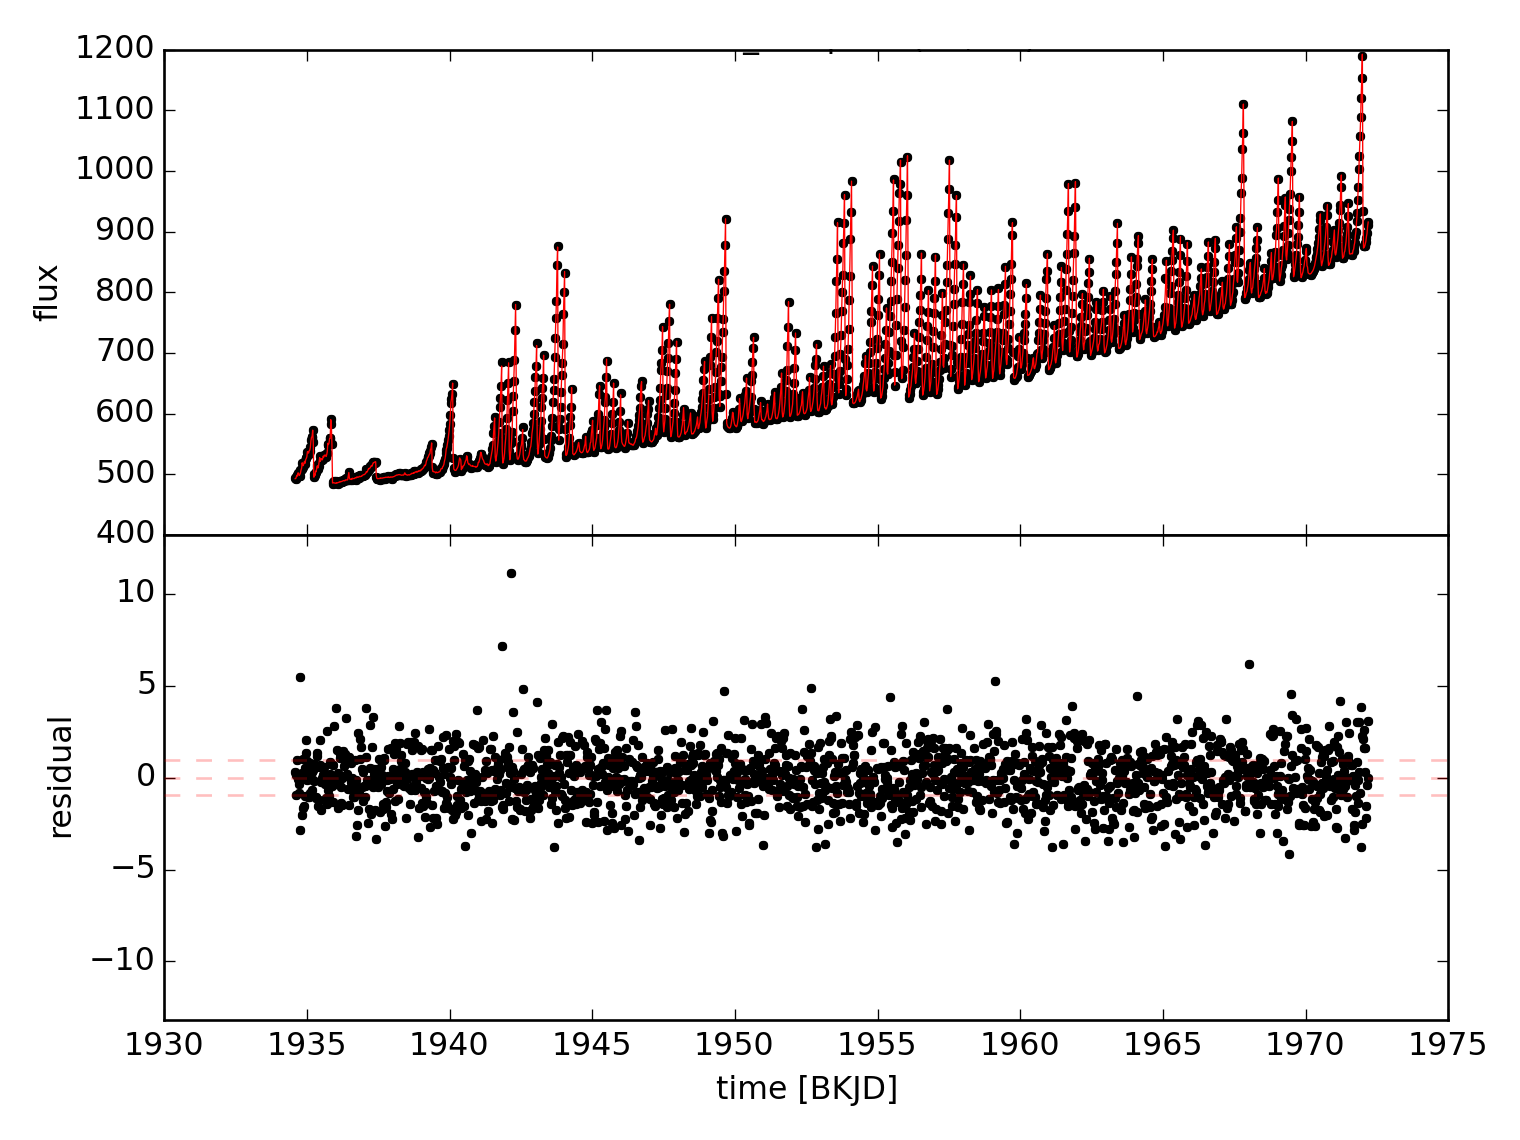
\includegraphics[width=0.49\textwidth]{f1a}
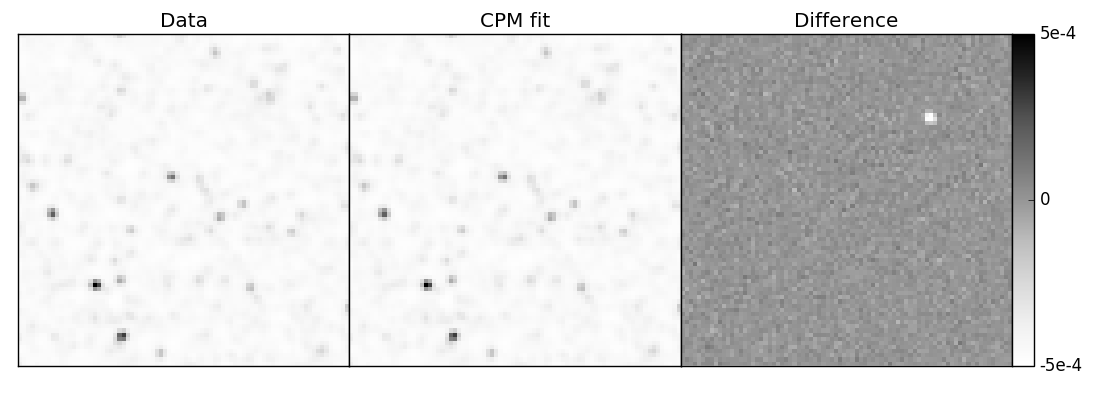
\includegraphics[width=0.49\textwidth]{f1b}
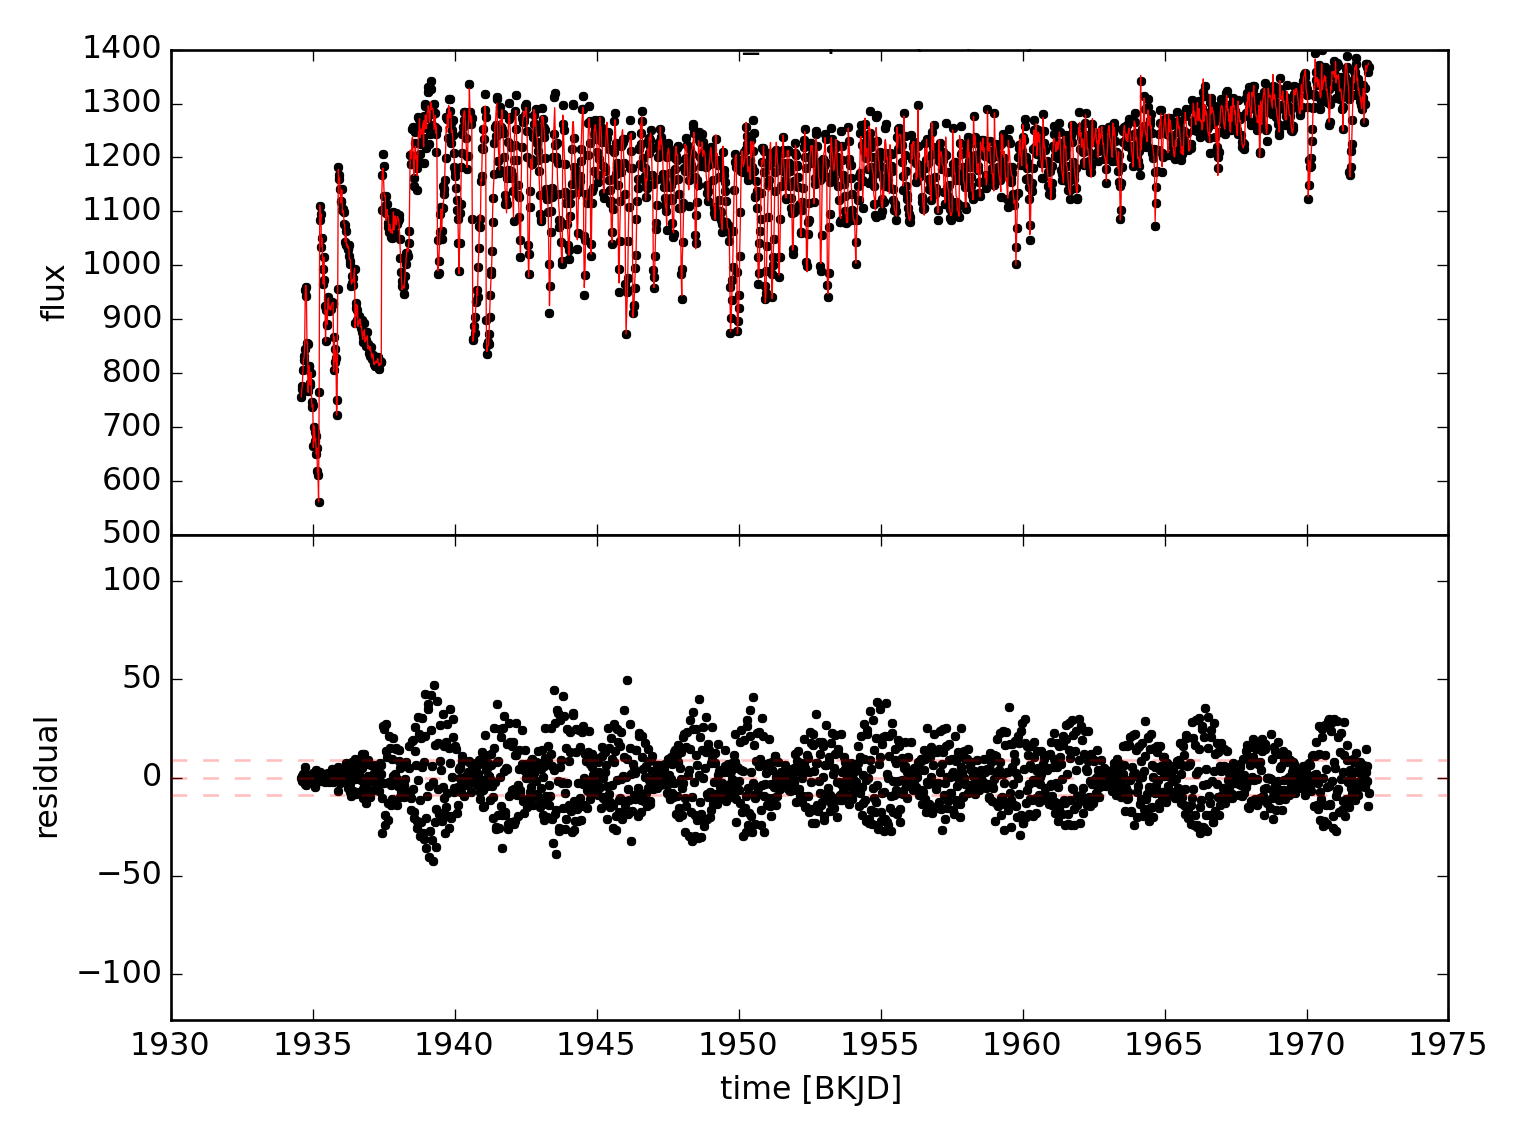
\includegraphics[width=0.49\textwidth]{f1c}
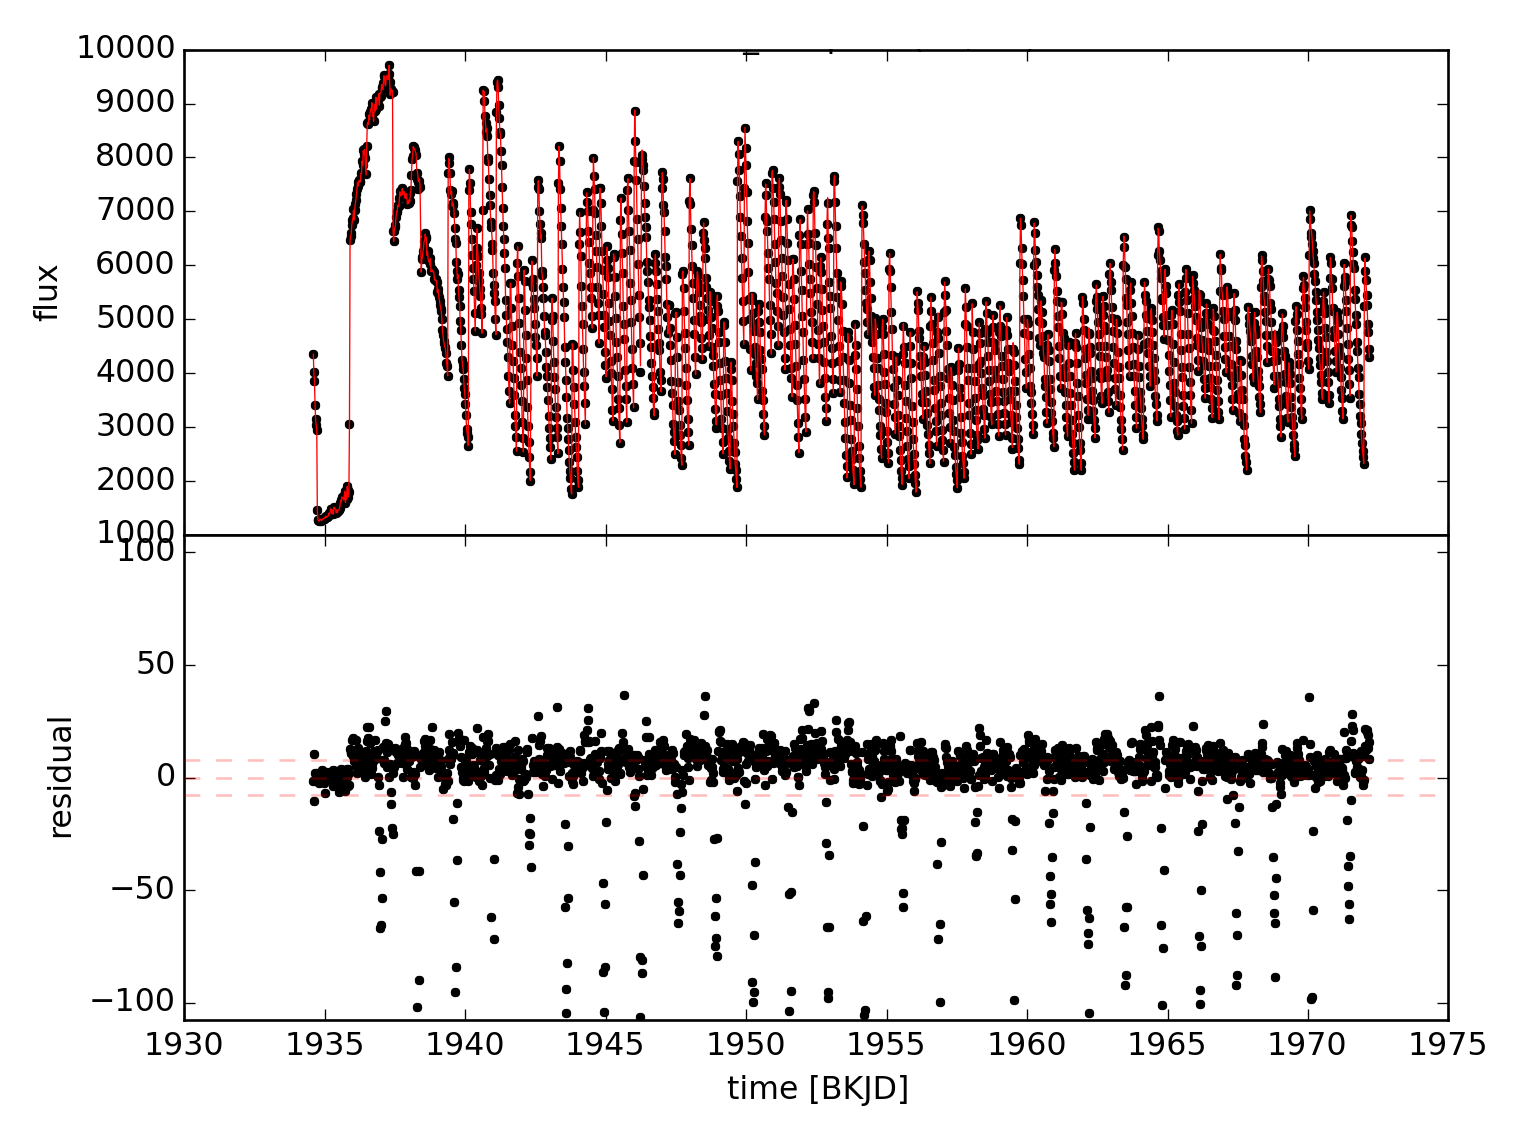
\includegraphics[width=0.49\textwidth]{f1d}

\end{center}

\caption{
  \label{lightcurves}
   The \cpm\ predcition of four pixels from \KTCZ. 
  Each plot shows the time series from one pixel.
  In the top panel of each plot, the black points are the pixel values over time from the data and the red lines are the prediction from the \cpm. 
  While in the bottom panel, the black points show the difference between data and prediction---the redsiduals and the three red lines indicate the mean and 1$\sigma$ variations.
  For pixels that do not contain variable sources (top two plots), the prediction perfectly agrees with the data and the residuals distribute normally around the zero. For pixels containing astronmical variabilities (bottom two plots), \cpm\ is still able to predict the systematic effects, while retain the astronmical variabilities.
}
\end{figure}


\begin{figure}[p]
\begin{center}
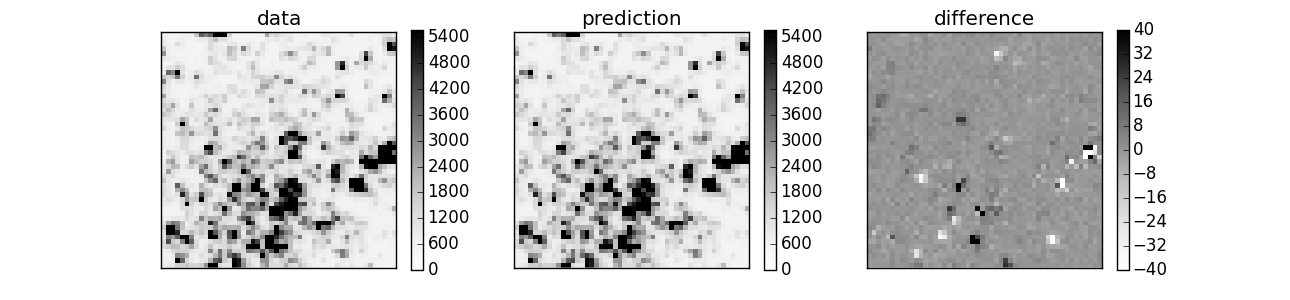
\includegraphics[width=0.96\textwidth]{f2a}
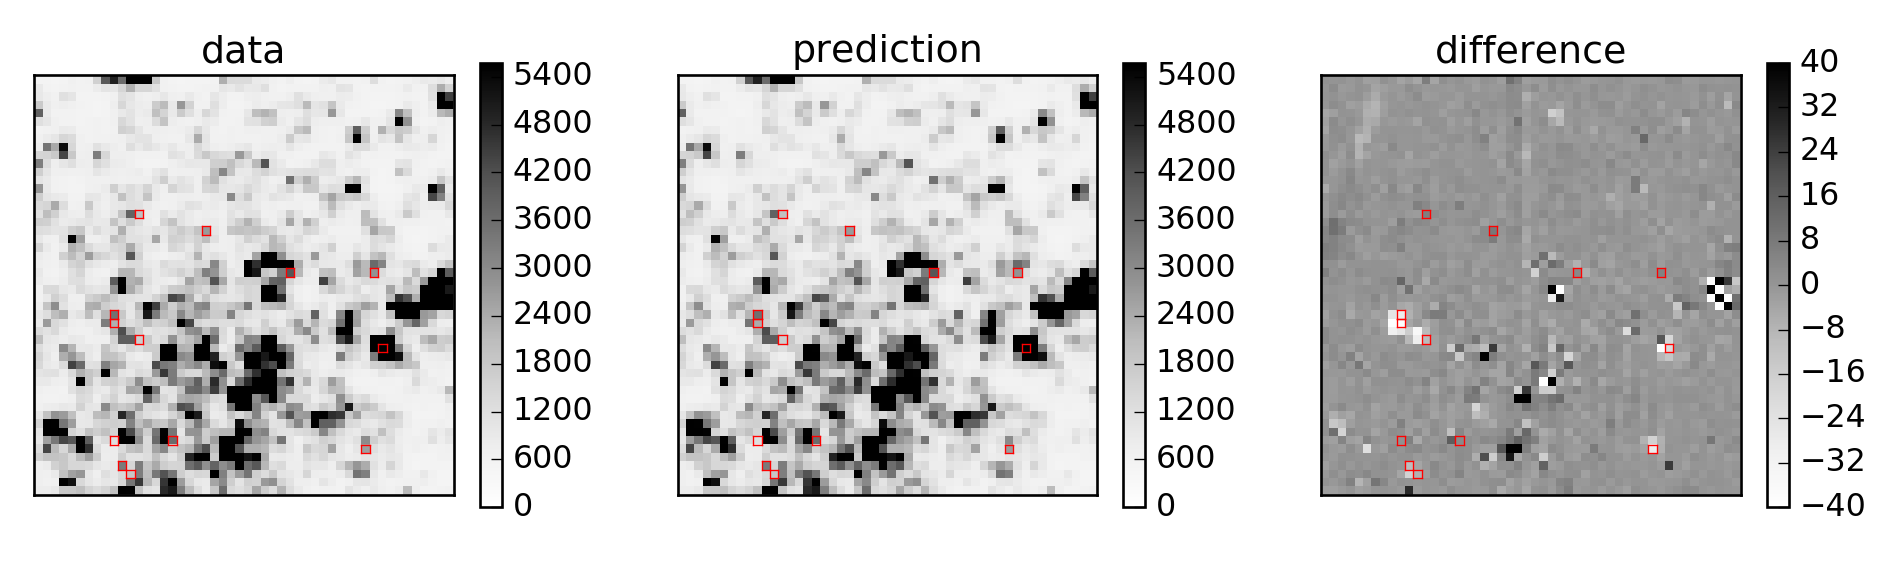
\includegraphics[width=0.96\textwidth]{f2b}
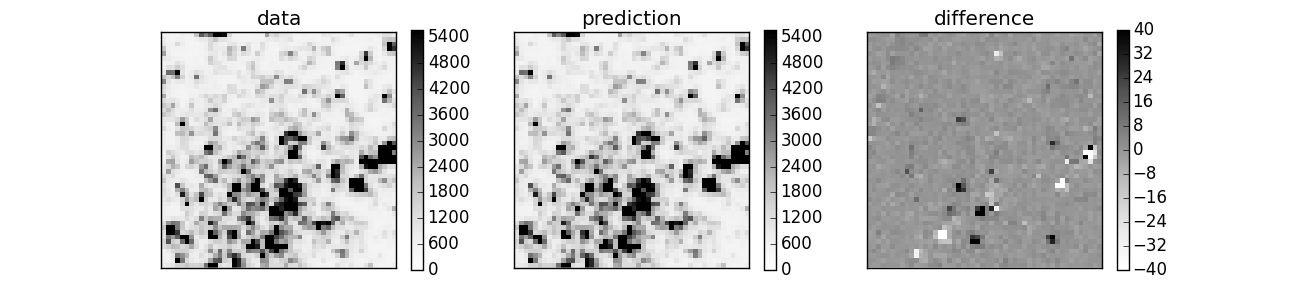
\includegraphics[width=0.96\textwidth]{f2c}
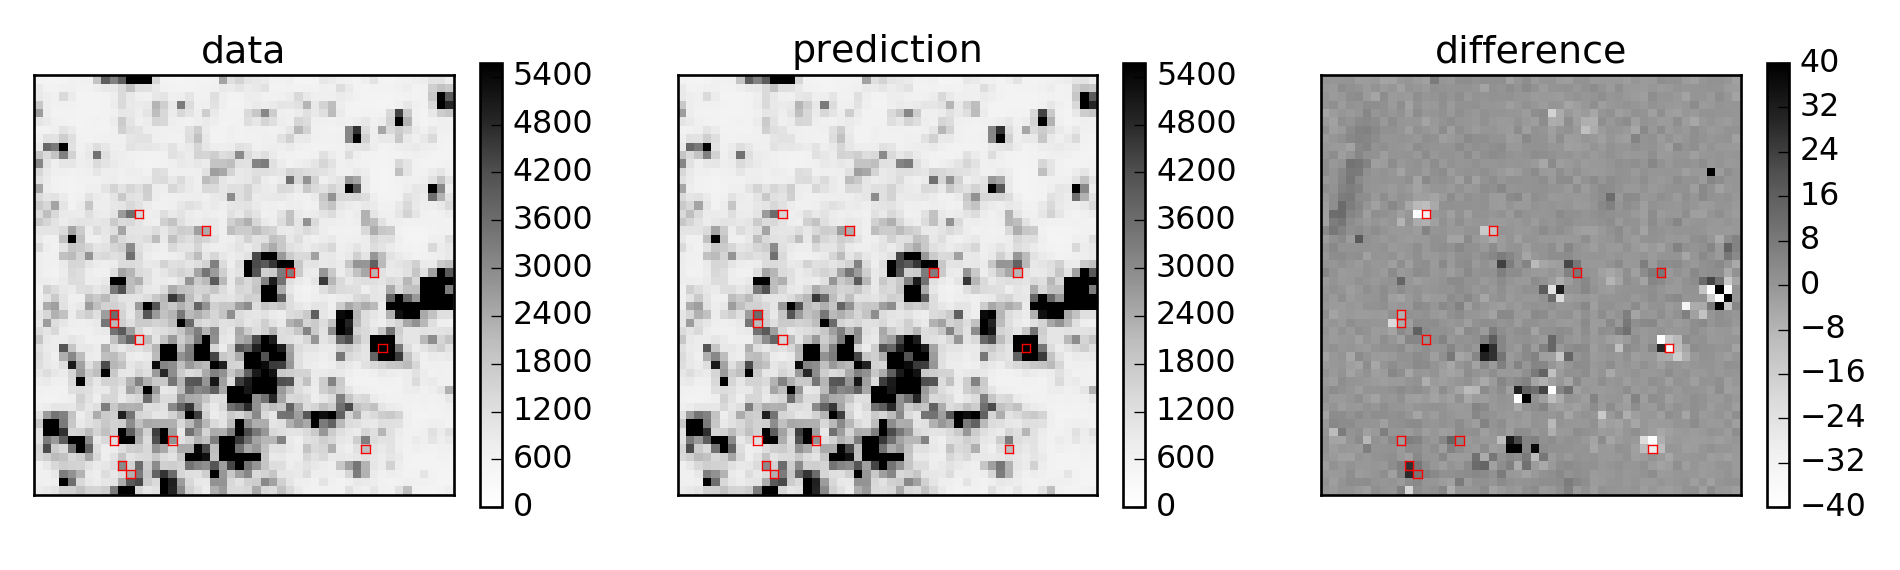
\includegraphics[width=0.96\textwidth]{f2d}

\end{center}
\caption{
  \label{images} 
  A $50\times50$ pixels image patch from \KTCZ. From top to the bottom,  each row shows a snapshot from different times.
  \emph{Left:} data from \KTCZ.
  \emph{Middle:} the prediction of the \cpmdiff.
  \emph{Right:} the difference between the data and the prediction.
  The pixels centered on the known variables from \cite{variables} are labeled by red boxes. 
  Most of the pixel values are around zero, except for few varible sources. which means the \cpmdiff\ can perfectly predict with the image data, while pull out the varibles.
}
\end{figure}

\begin{figure}[p]
\begin{center}
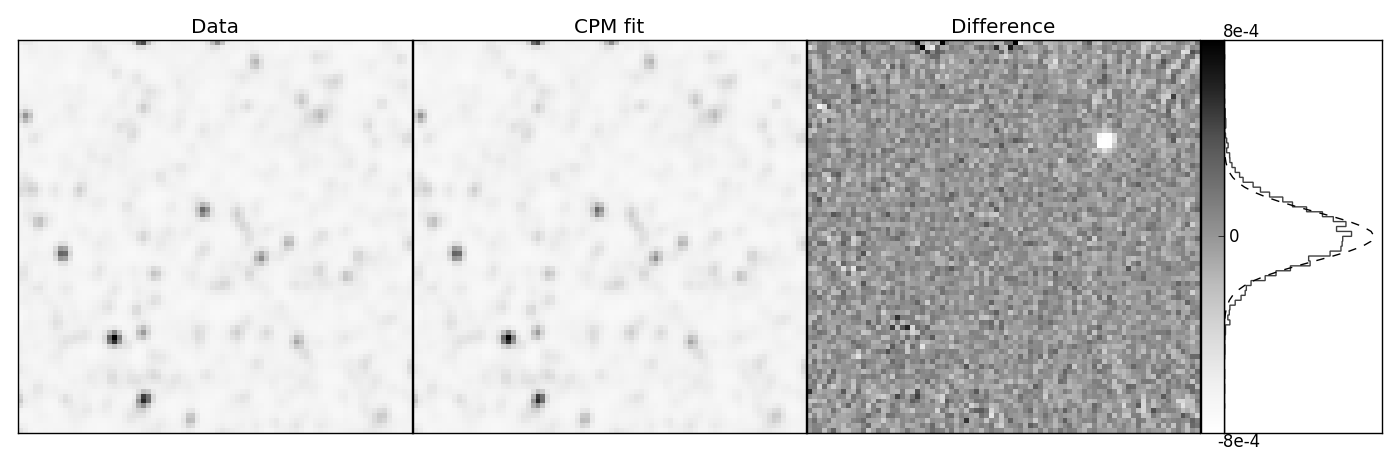
\includegraphics[width=0.32\textwidth]{f3a}
\hfill
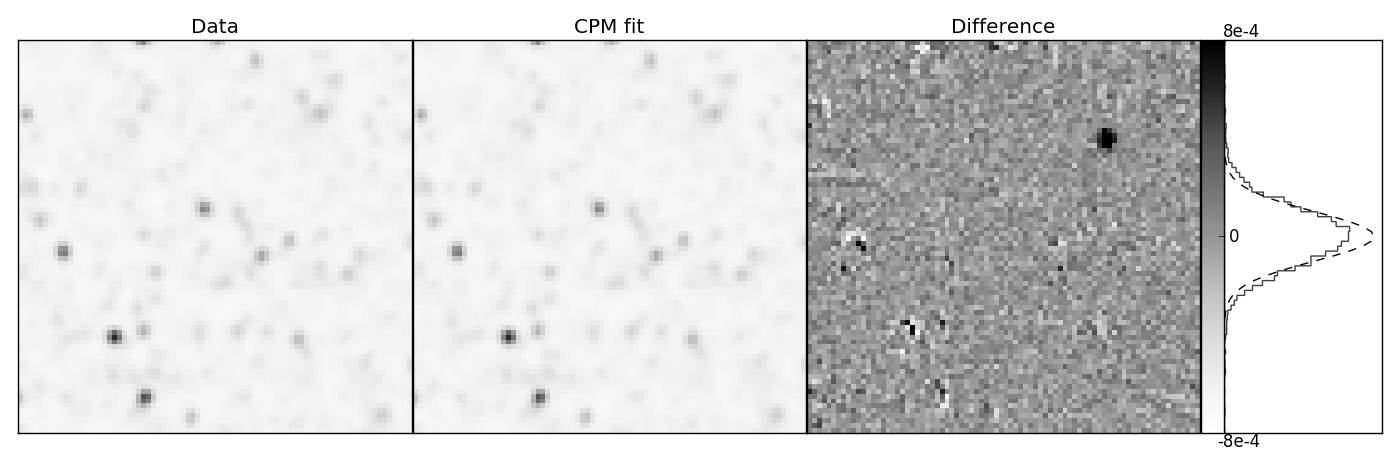
\includegraphics[width=0.32\textwidth]{f3b}
\hfill
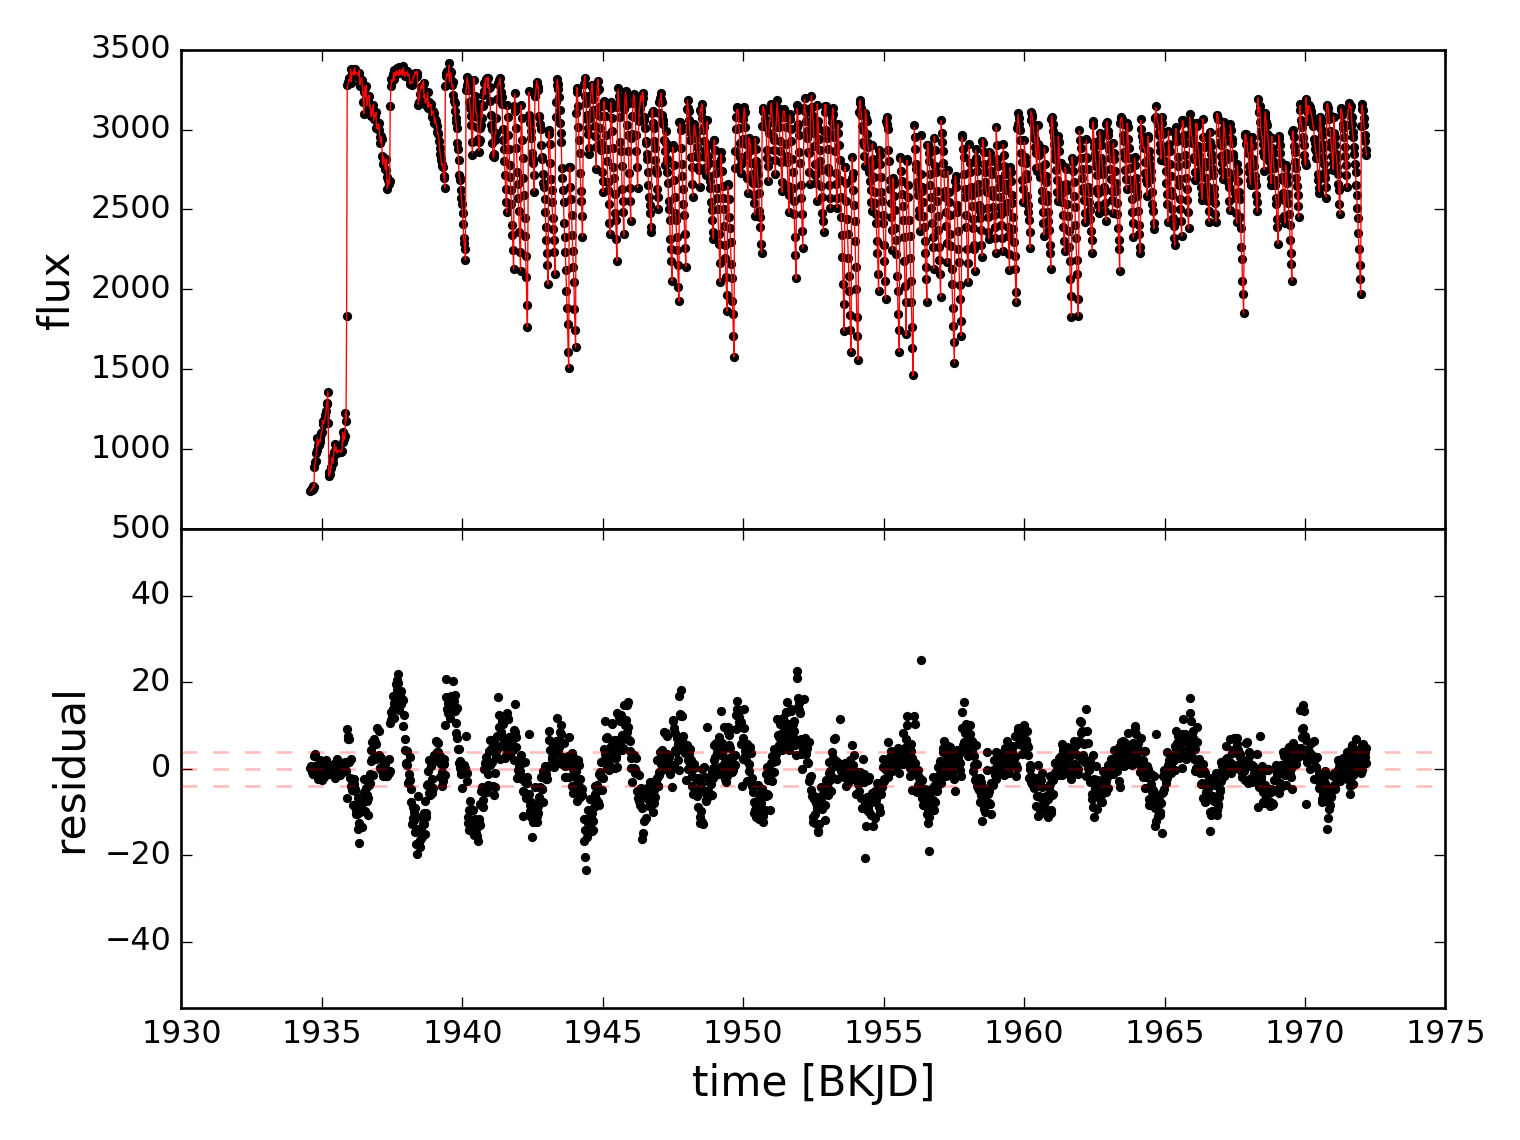
\includegraphics[width=0.32\textwidth]{f3c}

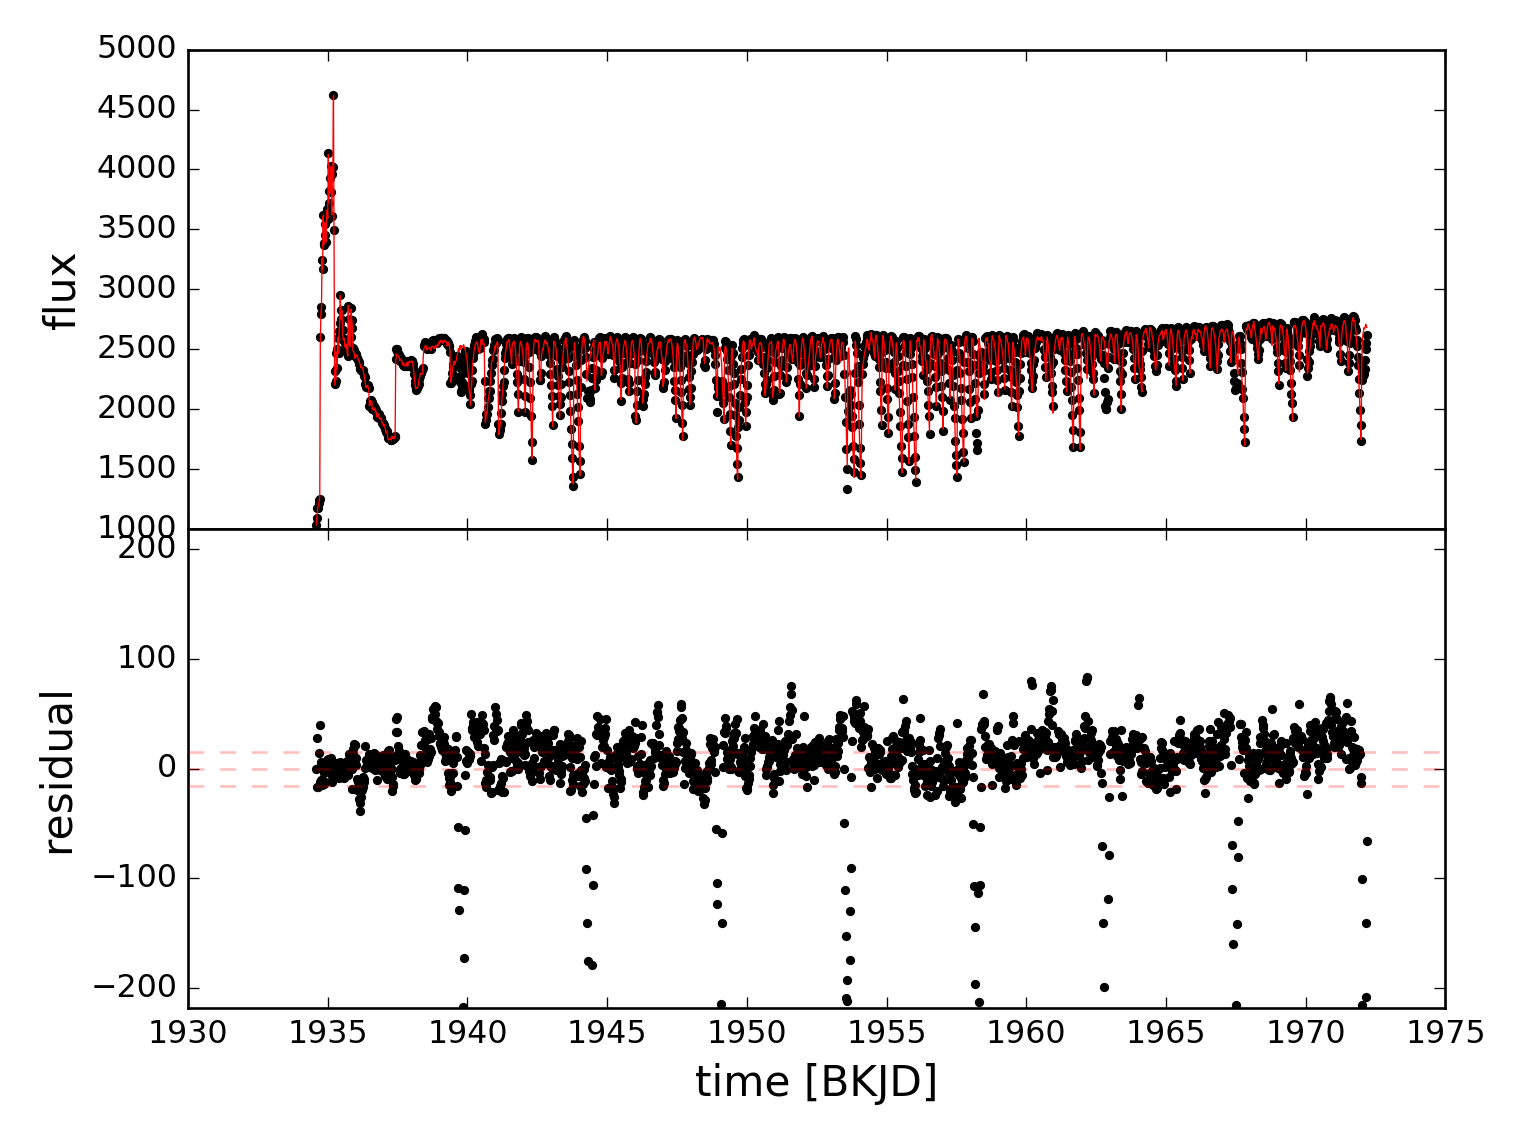
\includegraphics[width=0.32\textwidth]{f3d}
\hfill
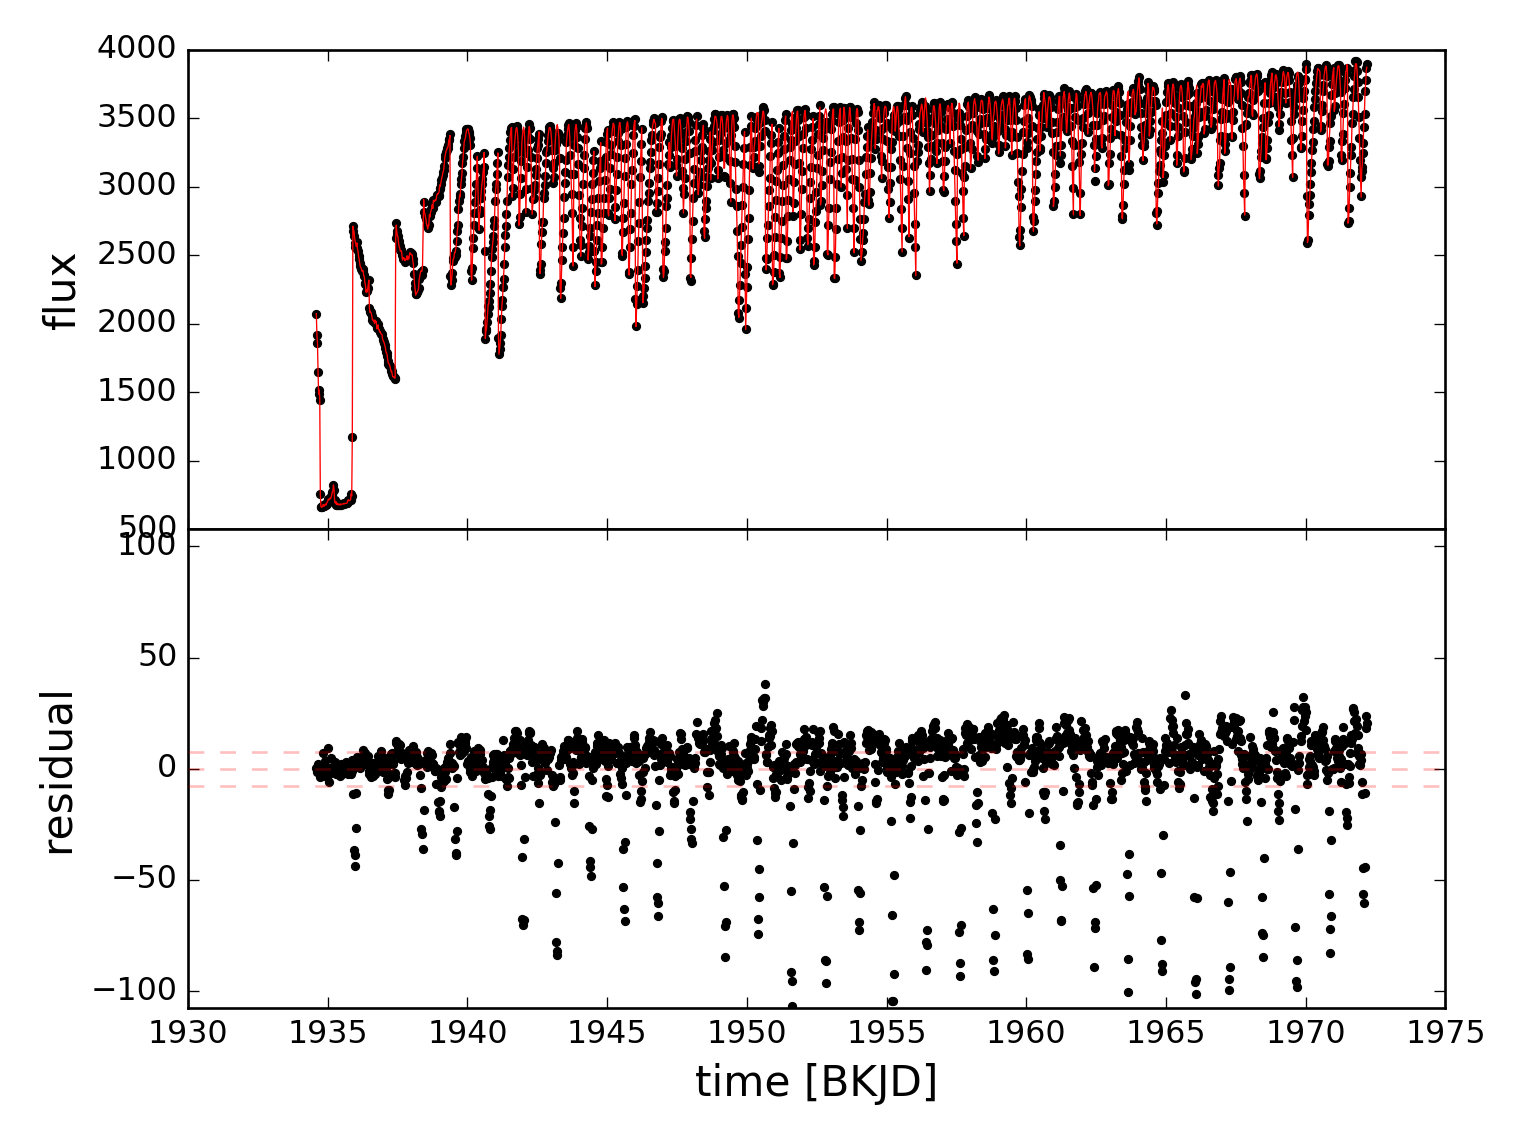
\includegraphics[width=0.32\textwidth]{f3e}
\hfill
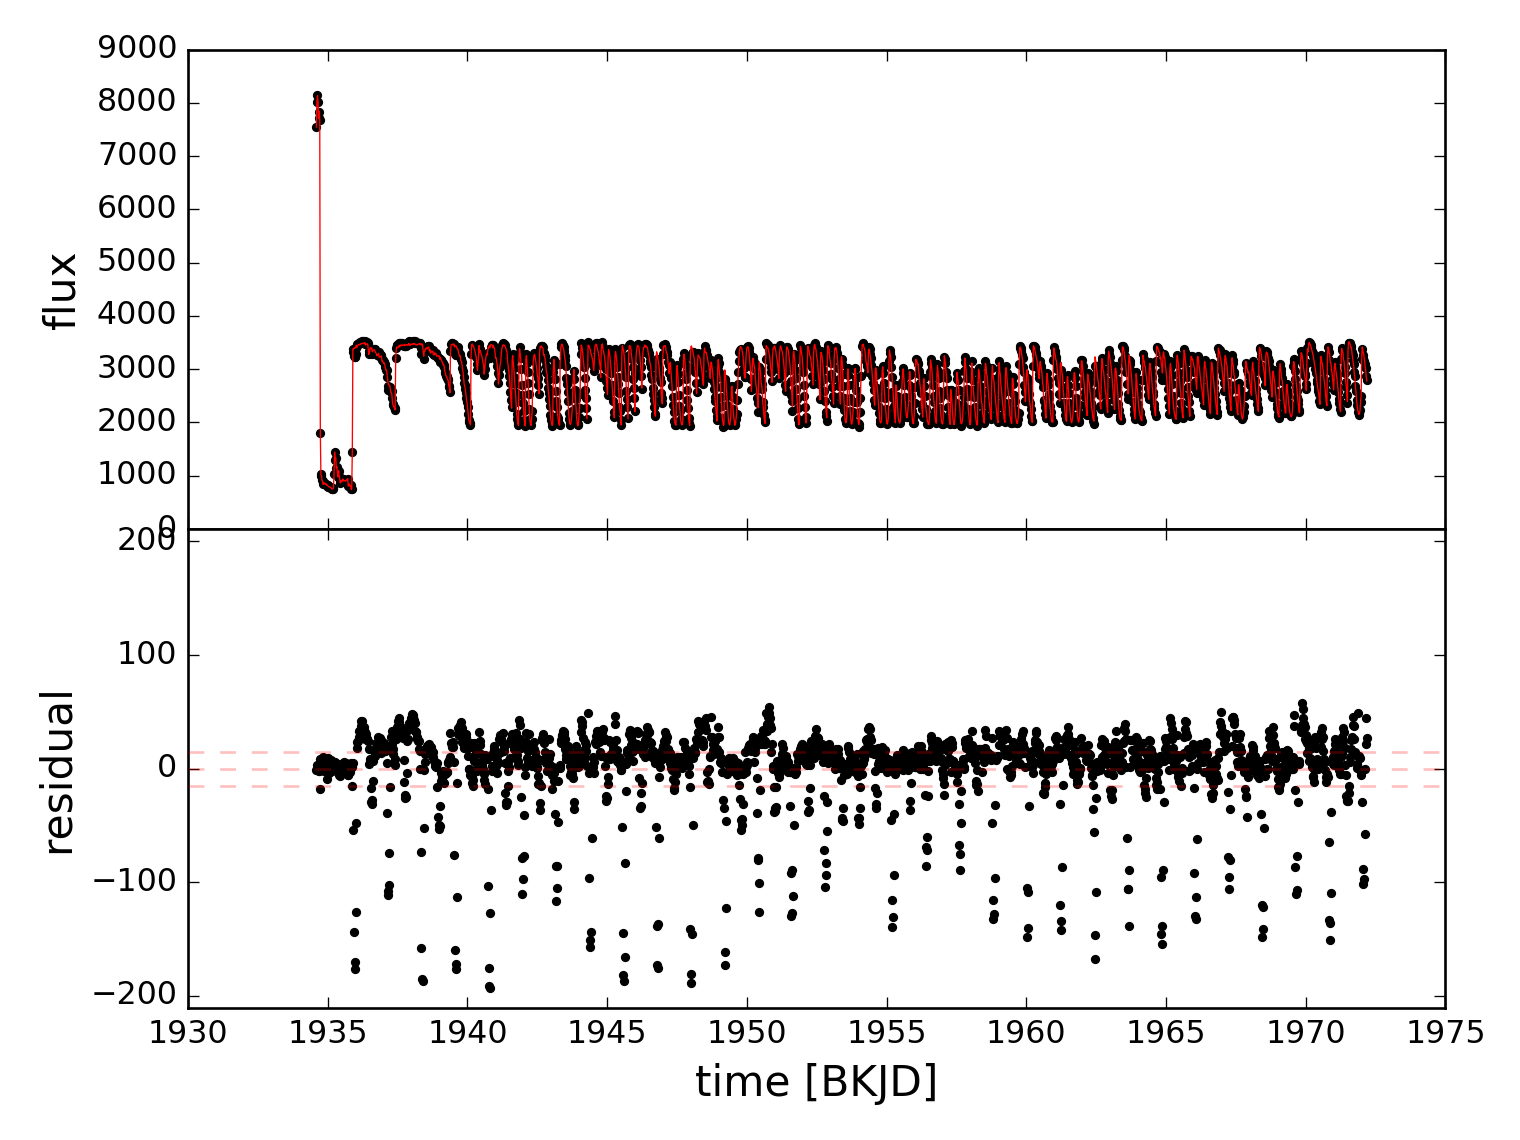
\includegraphics[width=0.32\textwidth]{f3f}

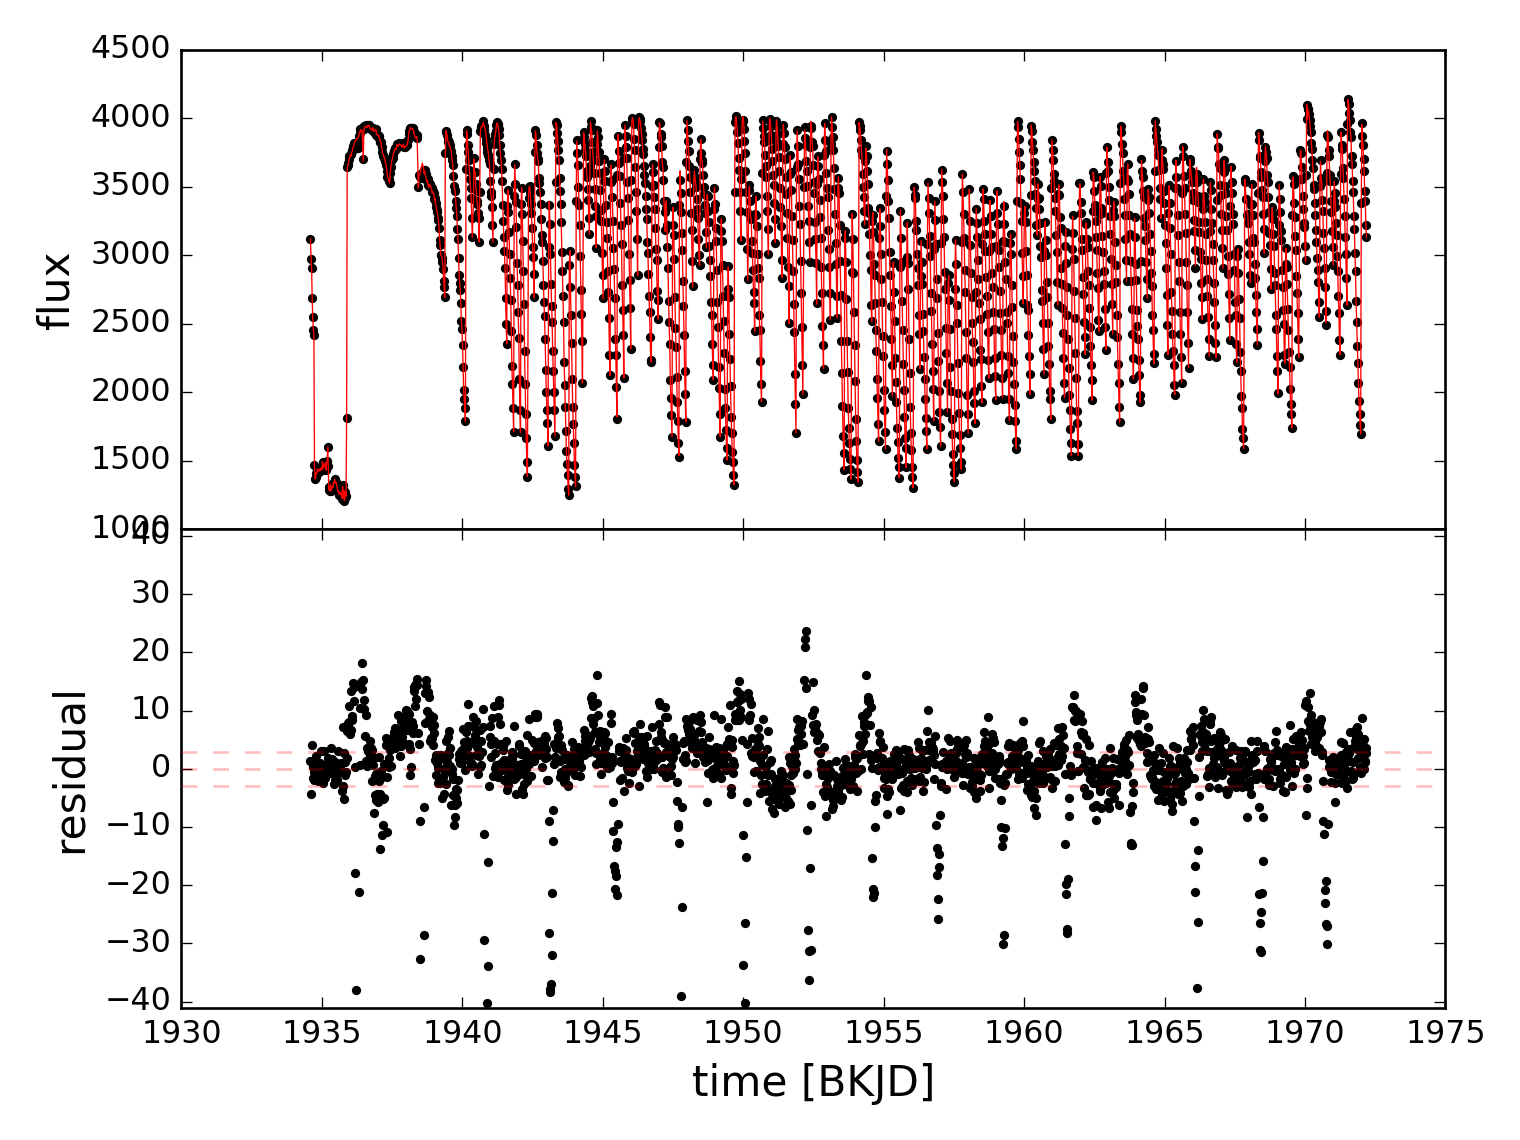
\includegraphics[width=0.32\textwidth]{f3g}
\hfill
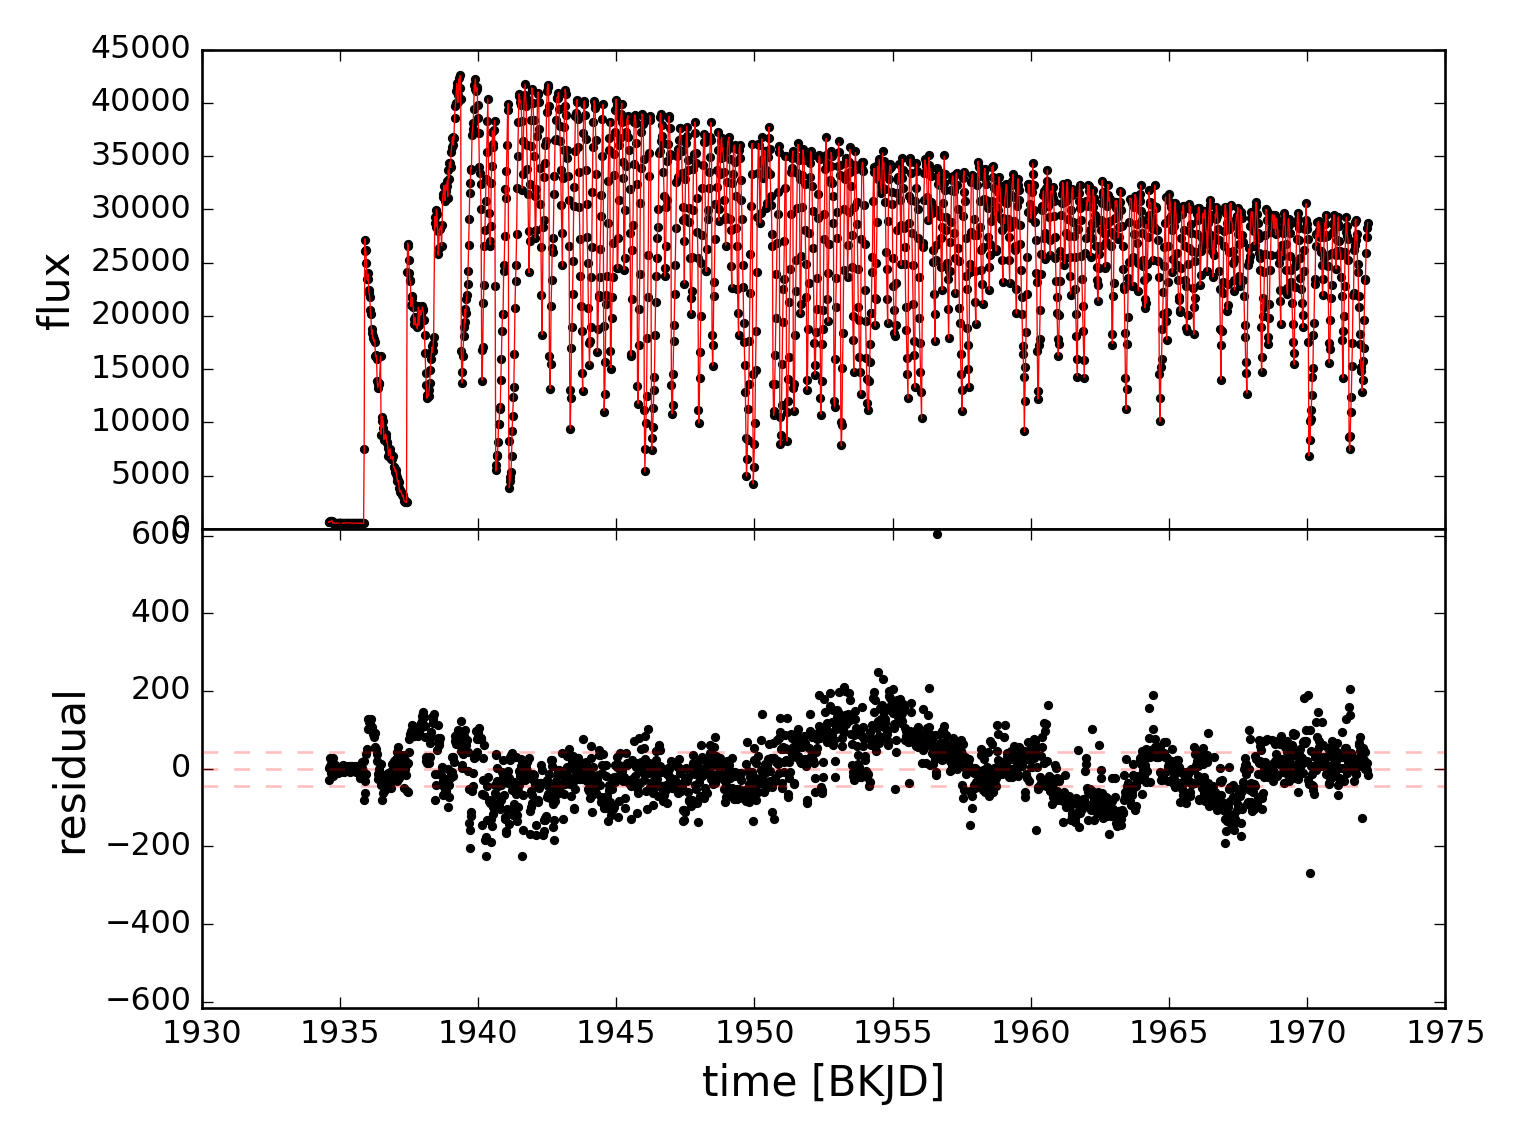
\includegraphics[width=0.32\textwidth]{f3h}
\hfill
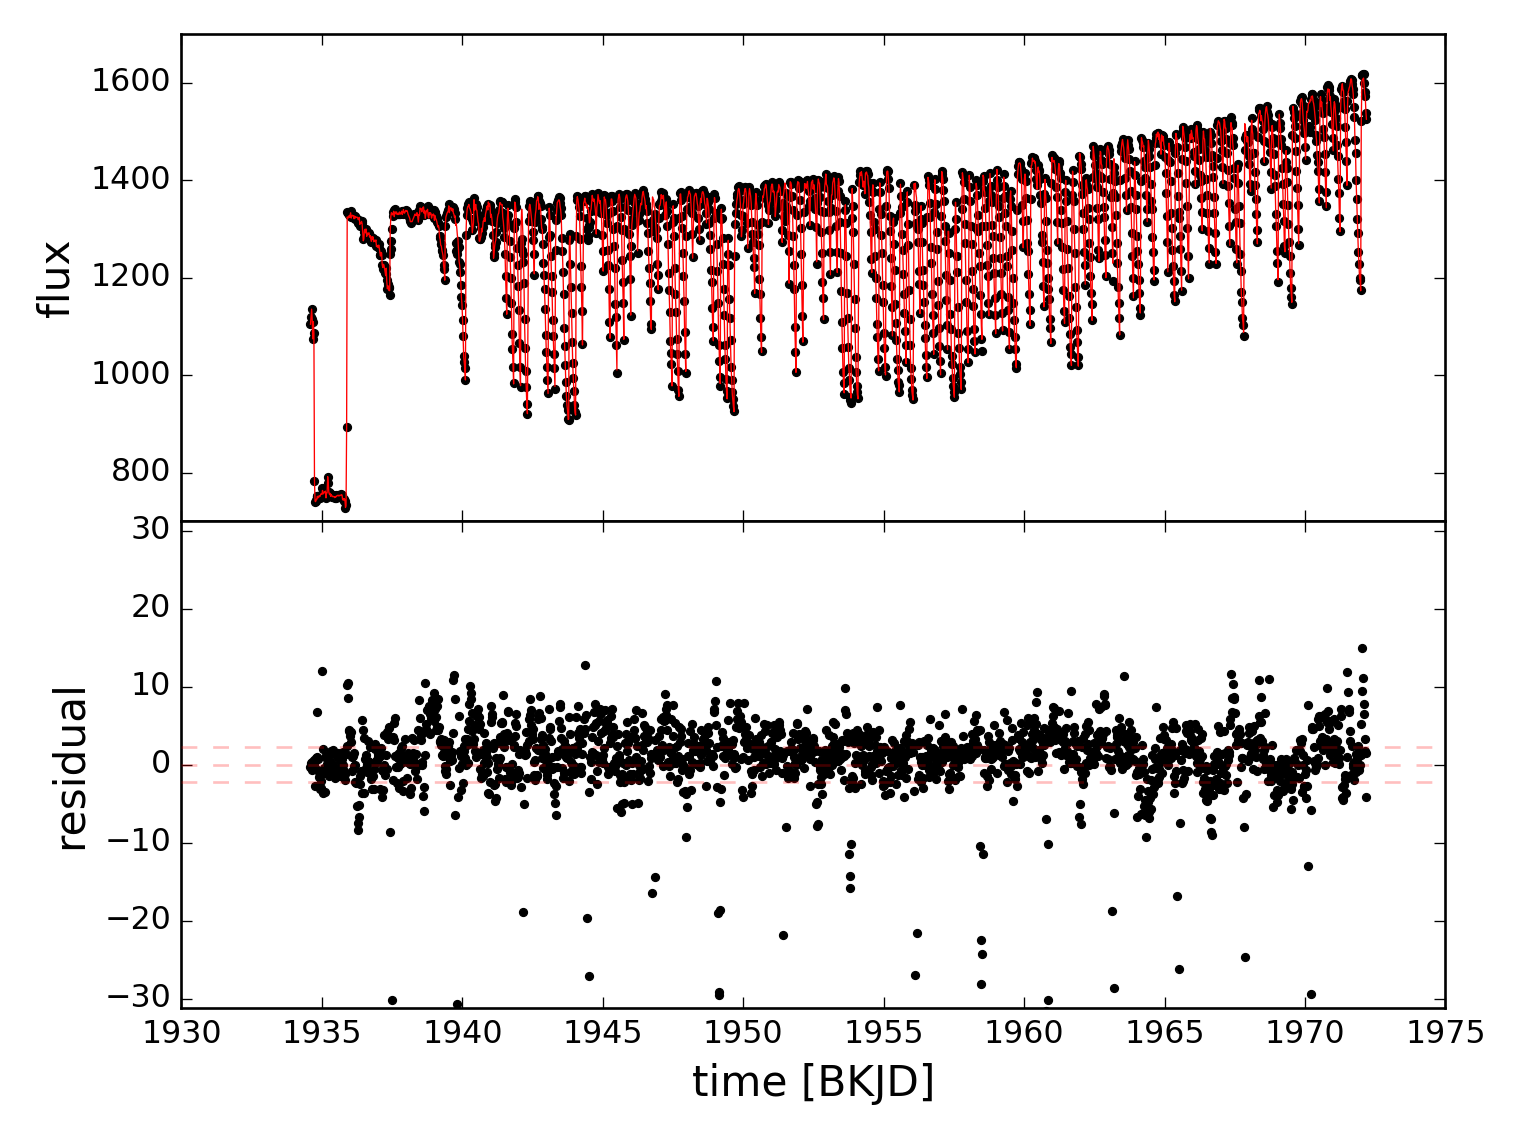
\includegraphics[width=0.32\textwidth]{f3i}

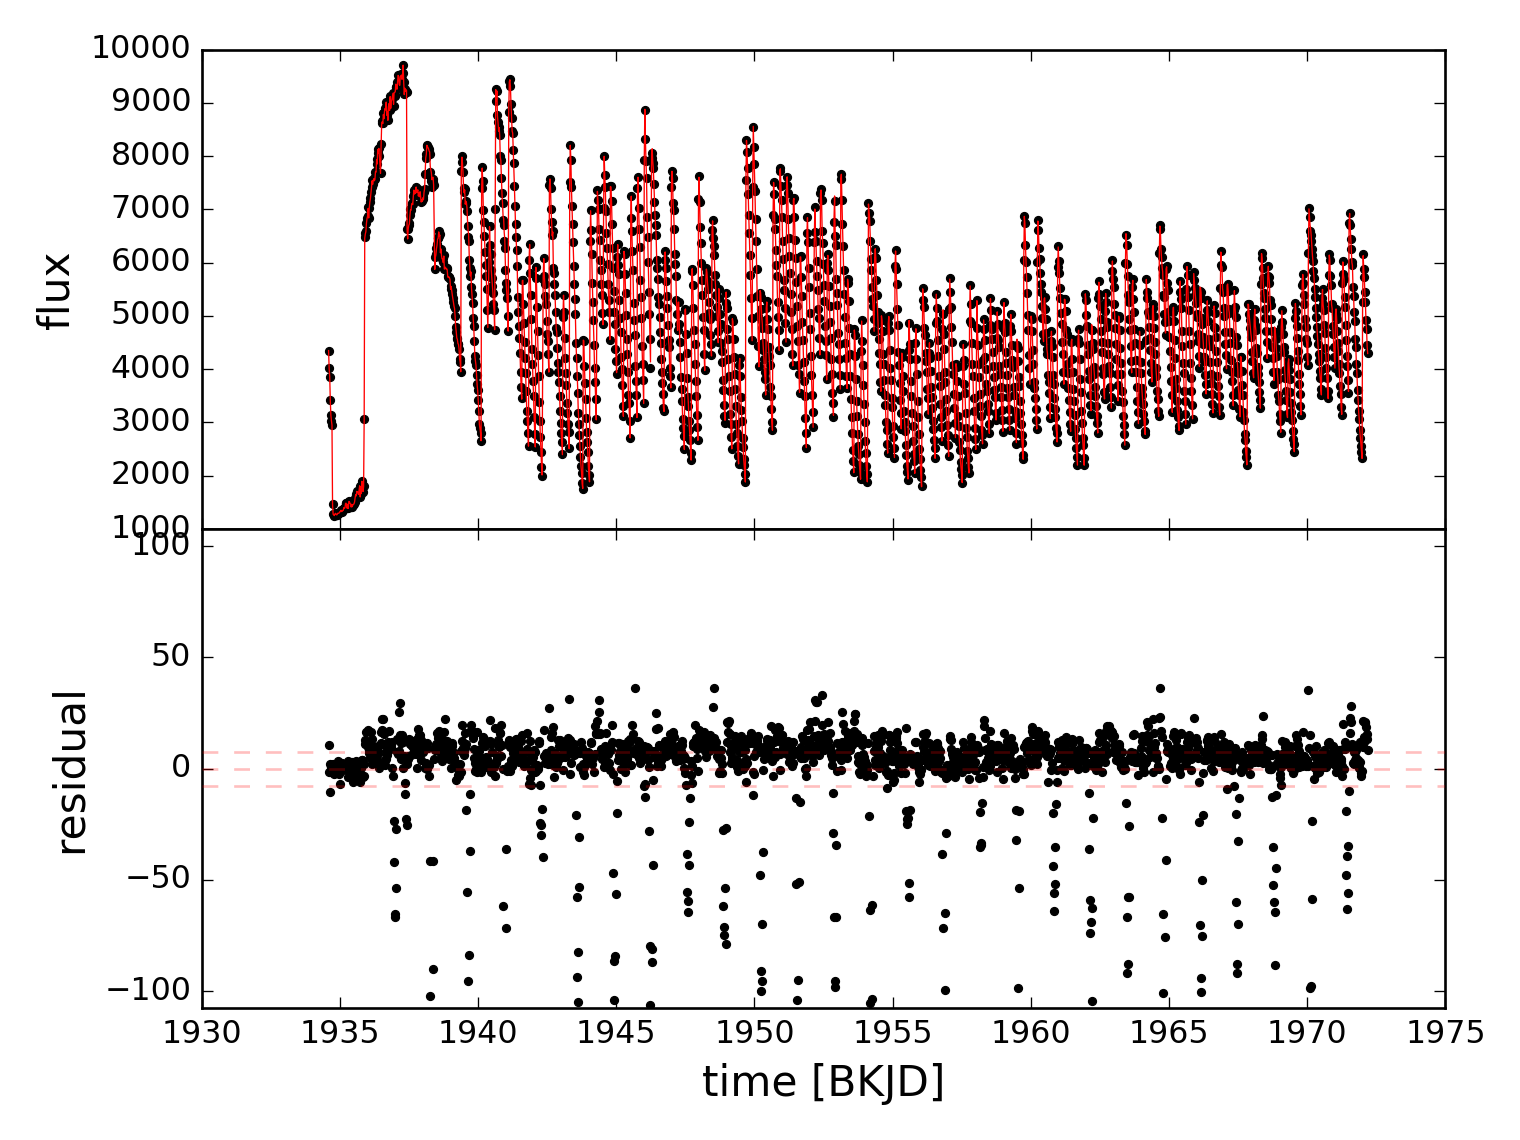
\includegraphics[width=0.32\textwidth]{f3j}
\hfill
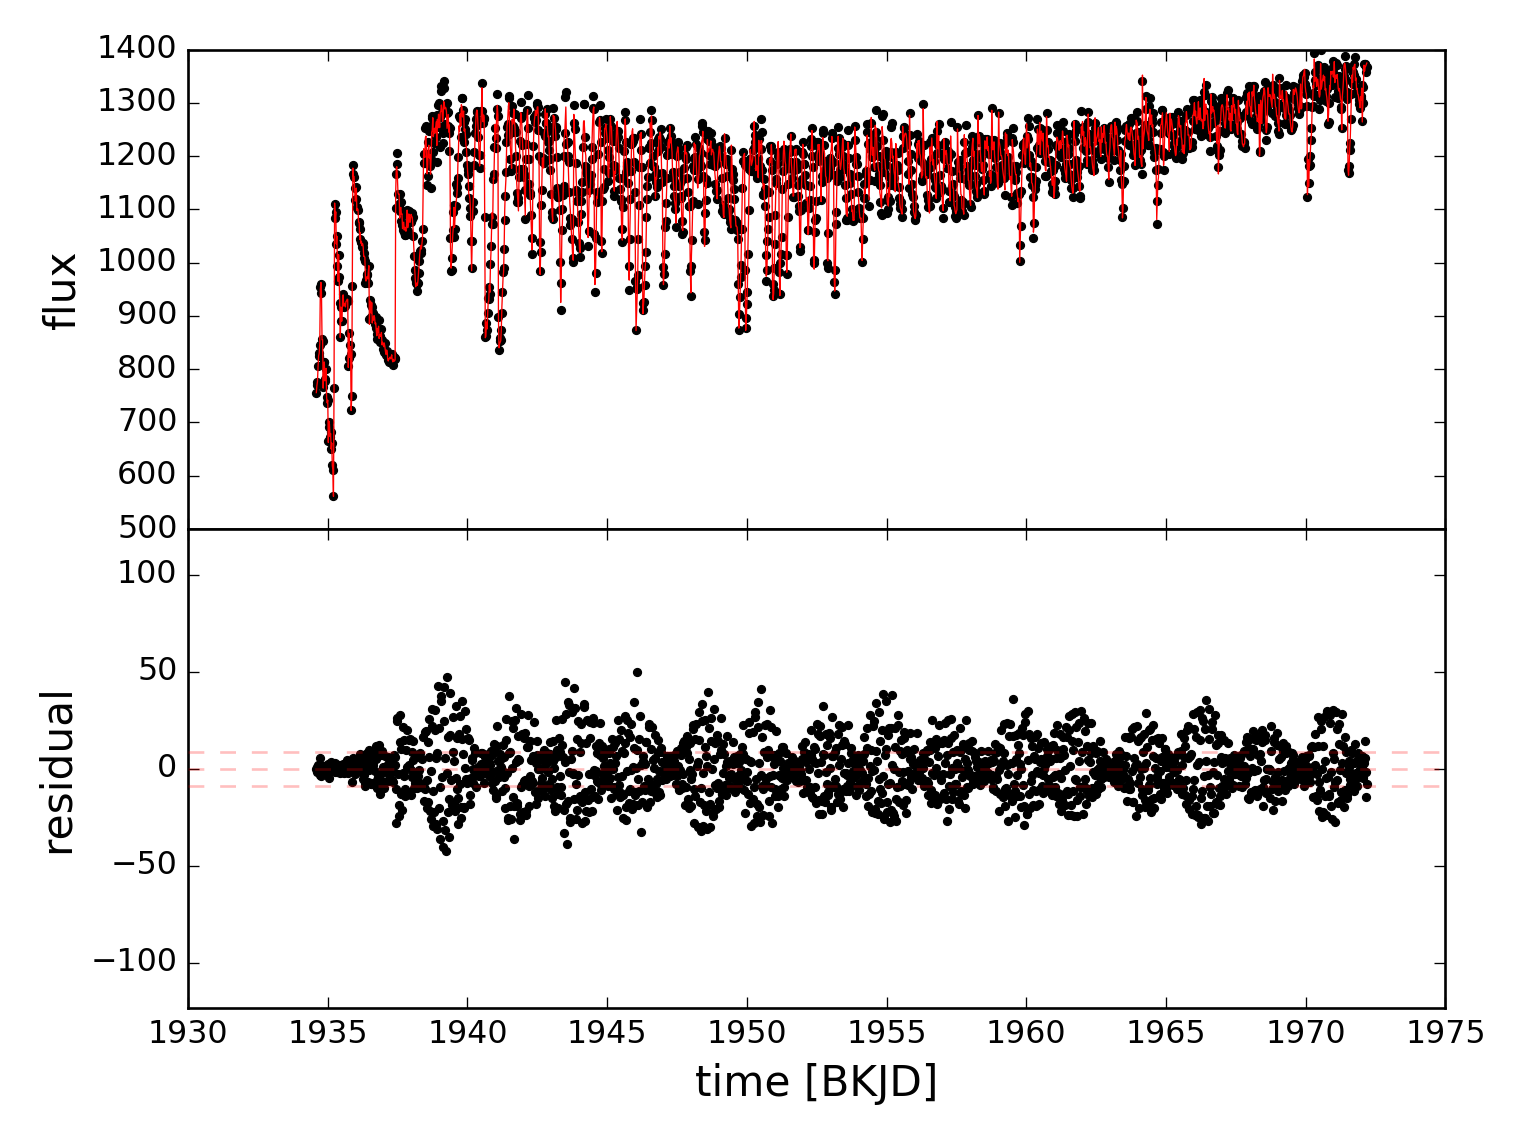
\includegraphics[width=0.32\textwidth]{f3k}
\hfill
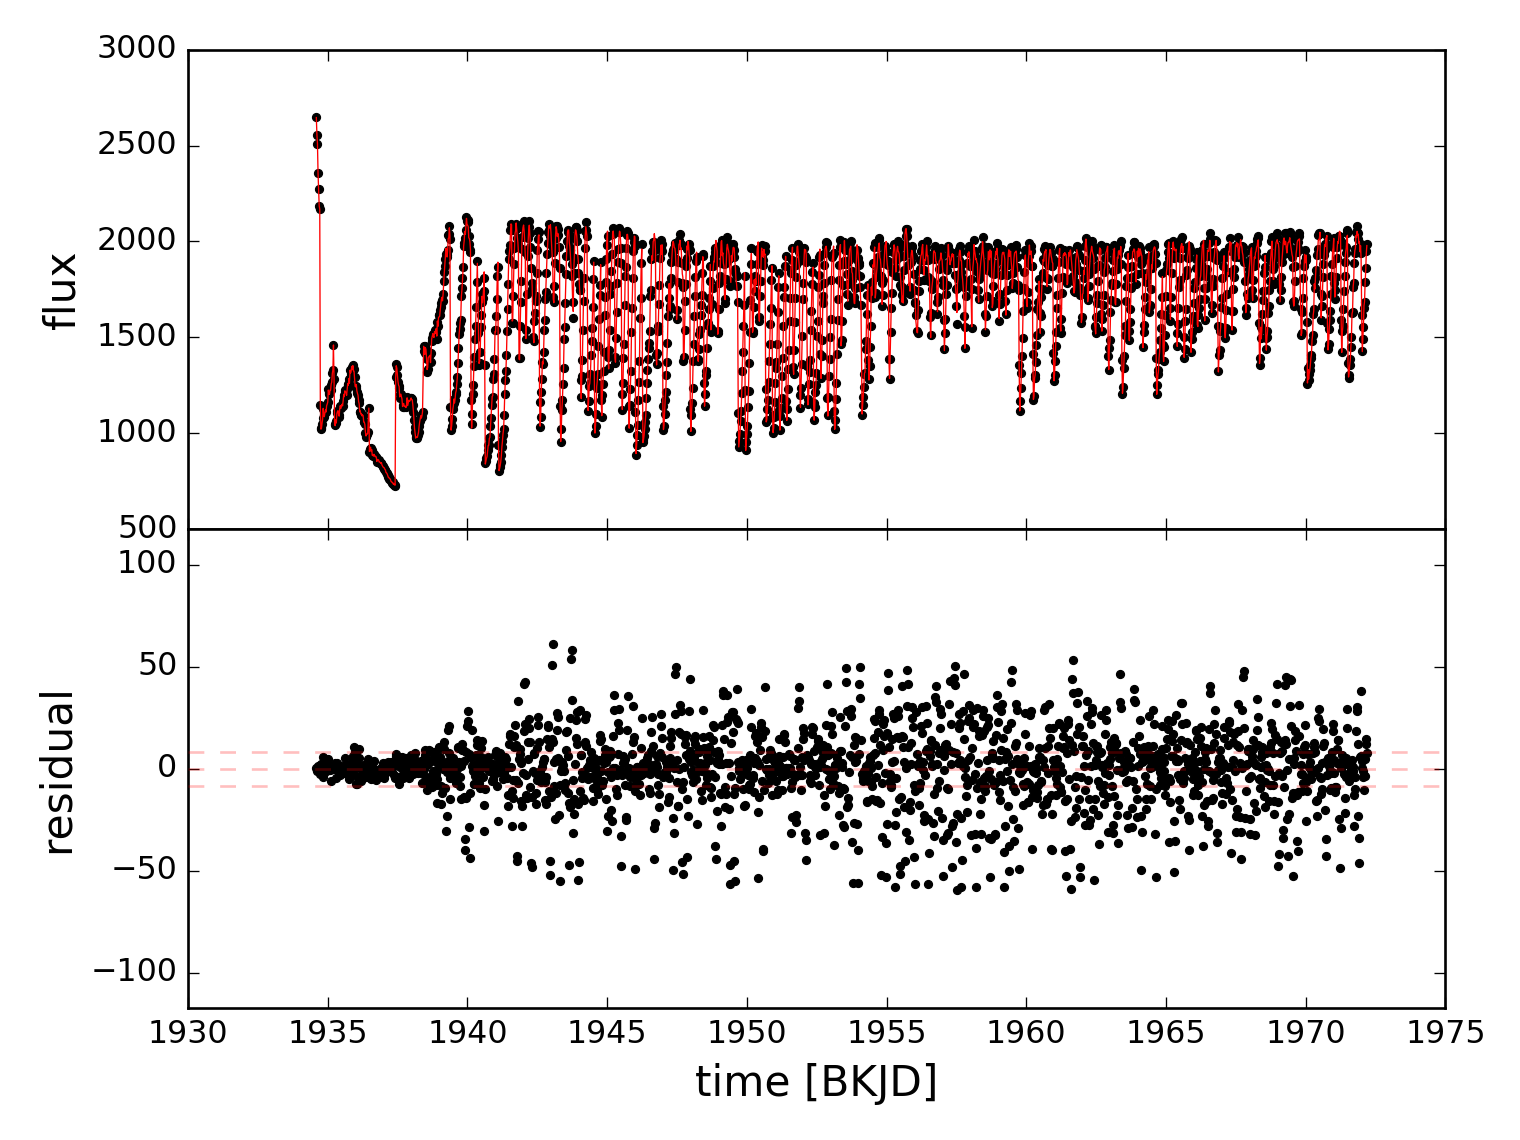
\includegraphics[width=0.32\textwidth]{f3l}
\hfill
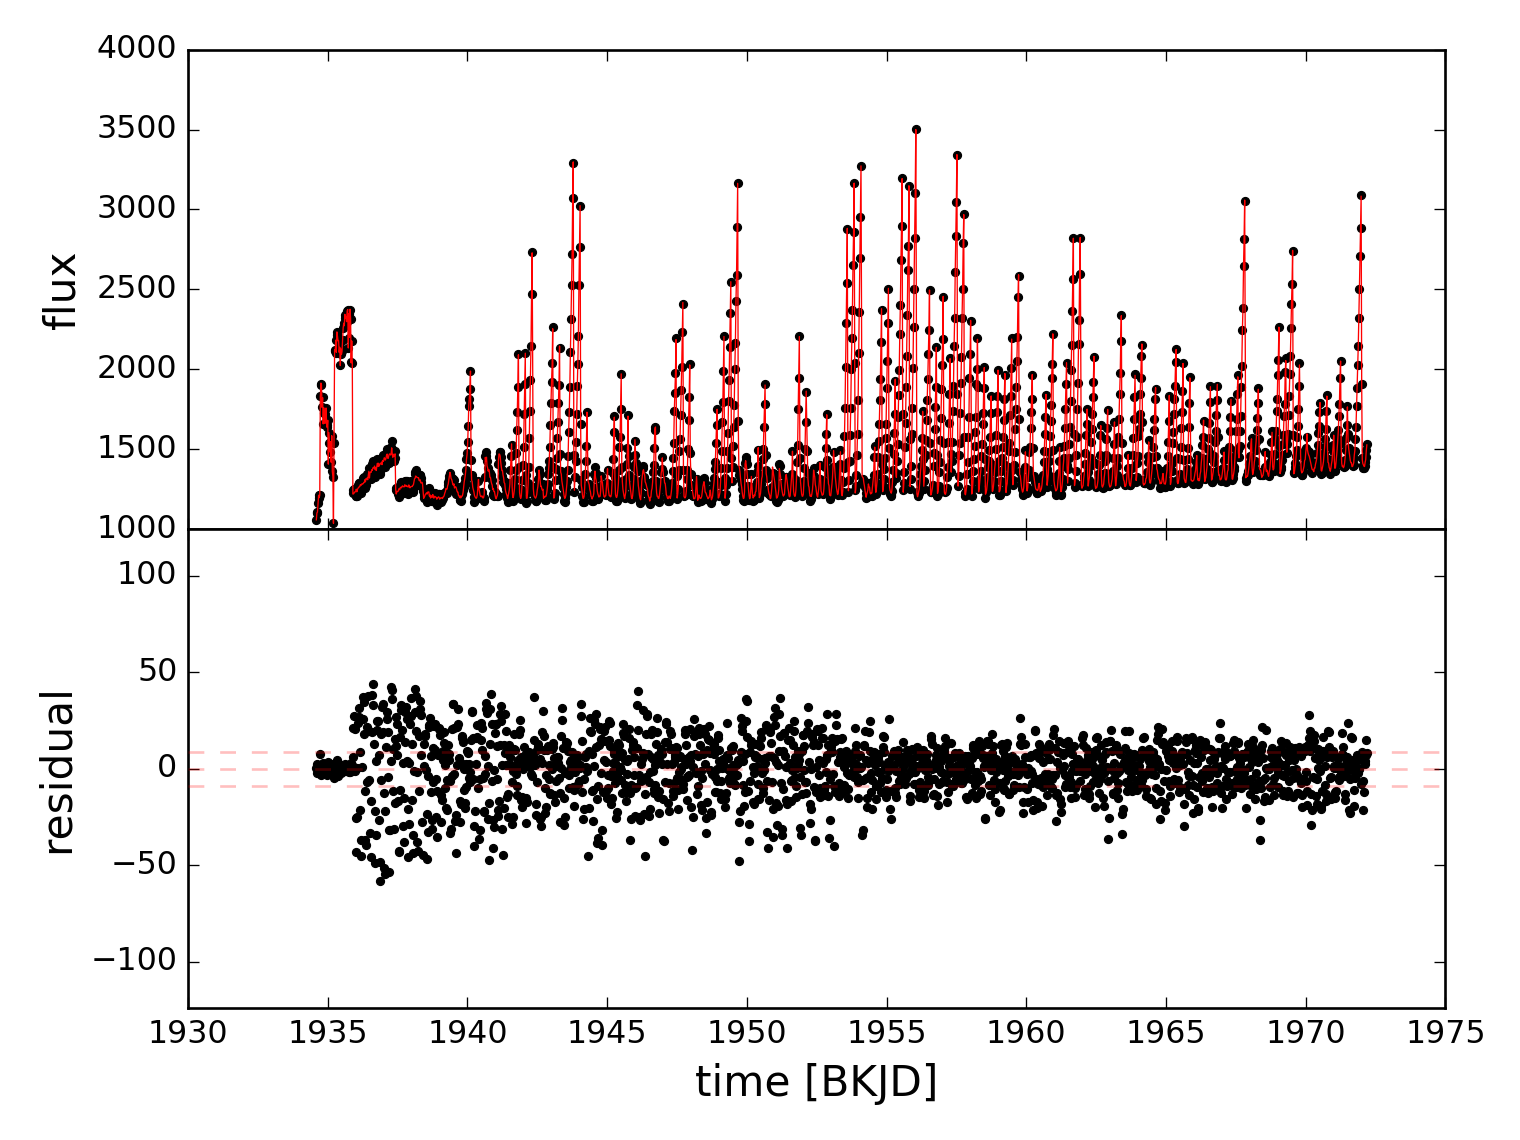
\includegraphics[width=0.32\textwidth]{f3m}
\end{center}

\caption{
  \label{variables} 
  The light curves of the pixels centered on known variables from \cite{variables}, which are labeld in Fig.~\ref{images}.
}
\end{figure}


\section{Discussion}
\todo{data taken differently}

\clearpage
\bibliography{cdi}
\clearpage

\end{document}